
\chapter{Estado del arte}
\label{cap:estado}
A la hora de tener una supervisión sobre la información producida a lo largo de un proceso productivo y poder tratarla a posteriorí, se usan sistemas software capaces de recopilar la información requerida en tiempo real del sistema y almacenarla para poder acceder a ella en un futuro.\\

Gracias a la informatización de la industria, estos sistemas están muy integrados dentro del proceso productivo puesto que, además de recopilar la información, se puede tener control directo en la producción. Una de las ventajas derivadas de la informatización, es que para tener el control del proceso, no es necesario encontrarse en el mismo lugar del mismo, gracias a Internet, se puede acceder desde cualquier parte del mundo y con cualquier dispositivo.\\

La palabra SCADA se usa para abreviar el término en inglés Supervisory Control And Data Adquisition o lo que es lo mismo, control supervisado y adquisición de datos. Un sistema SCADA puede ser utilizado en cualquer tipo de proceso en el cual se genere una cierta información que deba ser tratada por alguna persona, y se encuentre en un lugar remoto de la localización del proceso. En la Figura \ref{fig:smart_Controls} podemos observar un ejemplo de sistema SCADA orientado a la extrusión.

\begin{figure}[h!]
    \centering
    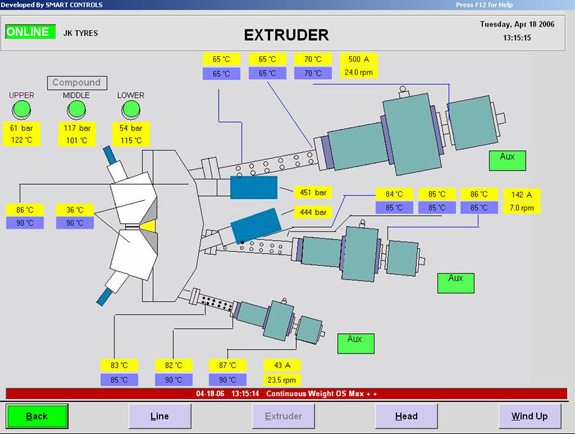
\includegraphics[width=0.6\textwidth]{images/triplex-extruder.jpg}
    \caption[Solución SCADA de la empresa SmartControls.]{Solución SCADA de la empresa SmartControls. Podemos apreciar como desde el sistema SCADA se accede a todas las variables que intervienen en el sistema. Fuente \cite{smartcontrols}.}
    \label{fig:smart_Controls}
\end{figure}

En lo referente a este tipo de aplicaciones, se han realizado avances y empresas como: Siemens, Wonderware, ABB o Rockwell Automation, ofrencen soluciones para implementar un sistema SCADA, y a día de hoy, prácticamente las soluciones son compatibles unas con otras.\\

Las distintas funciones que debe proveer un sistema SCADA son:

\begin{itemize}
    \item{Adquisición en tiempo real de los datos de intereses.}
    \item{Posibilidad de realizar gráficas de los datos adquiridos.}
    \item{Análisis de los datos obtenidos.}
    \item{Control sobre los distintos instrumentos del sistema.}
    \item{Acceso remoto al proceso productivo.}
\end{itemize}

Debido a la versatilidad de un sistema SCADA, son pocas las empresas que se dedican a una rama en concreto, se suele trabajar bajo pedido, y se diseñan sistemas SCADAS especificos para cada caso, sin embargo empresas como Castool ofrecen soluciones sistemas SCADA capaces de controlar totalmente el proceso productivo de la extrusión, Visual Optimizer \cite{castool}.\\

Castool ofrece un sistema de extrusión completo, suministrando tanto la maquinaría, software como personal cualificado para el uso de la línea de extrusión. Sin embargo esta solución solo sería útil en el caso que se adquiriera una línea de extrusión completa, en la mayoría de los casos no es lo habitual, puesto que siempre se suelen tener elementos de la linea de distintos fabricantes.\\

Son varios los fabricantes consolidados que proporcionan líneas de extrusión completas: Rondol, Everplast, Brabender, Labtech, entre otras; sin embargo buscando las soluciones SCADA que ellos proponen, no se ha encontrado en catálogo ninguna información al respecto.\\

En la Figura \ref{fig:extr_lyman} se muestra el extrusor Lyman, actualmente la solución mas aceptada en el ámbito de las extrusoras caseras.

\begin{figure}[h!]
    \centering
    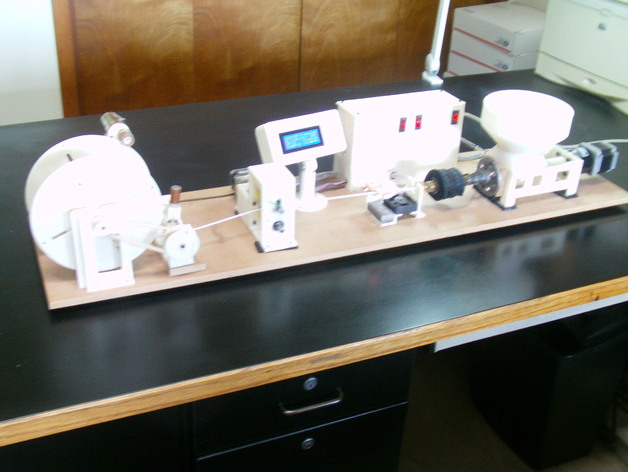
\includegraphics[width=0.6\textwidth]{images/lyman.jpg}
    \caption[Extrusor casero Lyman.]{Extrusor casero Lyman. Solución para fabricar una línea de extrusión completa de forma casera. Fuente \cite{lyman}.}
    \label{fig:extr_lyman}
\end{figure}

Esta solución provee un sistema completo de extrusión para que el usuario pueda fabricar su propio filamento de forma artesanal, incluyendo:

\begin{itemize}
    \item{Tolva para alimentar con pellets la extrusora.}
    \item{Extrusora de filamento.}
    \item{Sensor de diámetro final del filamento..}
    \item{Unidad tractora para ir desplazando el filamento extruido.}
    \item{Bobinadora automática para almacenar el filamento extruido.}
\end{itemize}

A pesar de que el control del extrusor Lyman es totalmente automático y sería fácil realizar un sistema de adquisición de datos, no se tiene constancia de que lo haya.\\

Debido a que la fabricación del filamento es un proceso novedoso, todos los sistemas que se han encontrado son relativos al control del flujo de material a través de la extrusora, ninguno incluye un sistema de gestión de calidad del filamento que se produce. Los sistemas actuales tampoco son lo suficientemente versatiles como para poder trabajar en cualquier línea de extrusión sin importar el fabricante de los distintos componentes que lo formen. Así mismo, todas las líneas de extrusión encontradas, incoroporan sistemas de visualización en tiempo real de los parámetros de producción sin posibilidad, de su registro en un medio físico para su posterior análisis de control de calidad.\\

El sistema que se propone en este trabajo final de grado suple esta necesidad, ya que se diseña desde un principio sin saber cual es el fabricante de la línea de extrusión final en el que se implementará. Así mismo, aunque el diseño incial del sistema es para controlar una única línea de extrusión, es totalmente escalabe para controlar varias líneas de extrusión al mismo tiempo.

